\documentclass{appolb}

\usepackage{ragged2e}
\usepackage{amsmath}
\usepackage{amssymb}
\usepackage{graphicx}
\usepackage{hyperref}
\usepackage{float}
\usepackage{caption}
\usepackage{subcaption}
\usepackage[
%backend=biber,
%style=ieee
maxbibnames=10,
%backend=bibtex,
natbib=true,
sorting=none
%backend=biber,
%style=apa
]{biblatex}
\addbibresource{./ref.bib}
\newcommand{\pairdot}[2]{ \mathbf{#1}\cdot\mathbf{#2}  }
\begin{document}
\title{Effects of the Sudakov form factor in the Golec-Biernat--W\"usthoff saturation model
\thanks{Presented at ``Diffraction and Low-$x$ 2022'', Corigliano Calabro (Italy), September 24-30, 2022.}
}
%\author{
%T.~Goda,$^1$, K.~Kutak$^{1,2}$ and S.~Sapeta$^1$\\\,\\
%$^1$ 
%{\small\it The H.\ Niewodnicza\'nski Institute of Nuclear Physics PAN,}\\ 
%{\small\it Radzikowskiego 152, 31-342 Krak\'ow, Poland}\\\,\\
%$^2$ 
%{\small\it Physics Department, Brookhaven National Laboratory,}\\
%{\small\it Upton, NY 11973, USA}\\
%}	 
\author{Tomoki Goda%, Sebastian Sapeta
\address{H. Niewodniczański Institute of Nuclear Physics,\\
	Radzikowskiego 152, 31-342 Cracow, Poland}\\
%	\vspace{3mm}
%	Krzysztof Kutak
%\address{ Physics Department, Brookhaven National Laboratory,\\
%Upton, NY 11973, USA\\
%H. Niewodniczański Institute of Nuclear Physics,\\
%	Radzikowskiego 152, 31-342 Cracow, Poland}\\
%Sebastian Sapeta
%\address{H. Niewodniczański Institute of Nuclear Physics,\\
%	Radzikowskiego 152, 31-342 Cracow, Poland}\\
}
%\address{
%in collaboration with K.~Kutak, S.~Sapeta
%}
%}
\maketitle
\begin{abstract}
We incorporate  the Sudakov form factor into the Golec-Biernat--W\"usthoff and Bartels--Golec-Biernat--W\"usthoff saturation models. The parameters are fitted to the HERA data. Both the models show considerable improvements in the fit quality.
\end{abstract}
\section{Introduction}
In the dipole picture of Deep Inelastic Scattering~(DIS), one can factorize the scattering cross section into the photon wave function $\Psi(z,x,Q)$ which describes the fluctuation of a photon with virtuality $Q^2$ splits into a quark--anti-quark pair with light-cone momentum fractions $z$ and $1-z$ respectively, and the dipole cross section $\sigma_\mathrm{dipole}(x,r)$ which describes the interaction of the $q\overline{q}$ pair of size $r$, with the proton~\cite{Golec-Biernat:1998zce, Kovchegov:2012mbw}. One may obtain $\sigma_\mathrm{dipole}$ from appropriate evolution equations such as Balitsky--Kovchegov~\cite{Balitsky:1995ub,Kovchegov:1999yj}
, however it is often useful to have a simple model.
The dipole cross section and the dipole unintegrated gluon distribution, $\mathcal{F}(x,k_t^2)$, are related to each other by~\cite{Golec-Biernat:1999qor,Bartels:2002cj}
\begin{align} 
    \sigma_{\mathrm{dipole}}(x,r) &= \frac{4 \pi}{N_c} \int\frac{d^2 \mathbf{k}_t }{k_t^2} \alpha_s \mathcal{F}(x, k_t^2) (1-e^{i {\mathbf{k}_t\cdot \mathbf{r}}}),
    \label{eq:ugdtosigma}\\
    \alpha_s \mathcal{F}(x,k_t^2) &= \frac{N_c }{4 \pi}\int \frac{d^2  \mathbf{r}}{(2\pi)^2} e^{i {\mathbf{k}_t\cdot \mathbf{r}}}  \nabla^2_{\mathbf{r}} \sigma_{\mathrm{dipole}}(x,r).
    \label{eq:sigmatougd}
\end{align}
We use these relations to incorporate the Sudakov form factor in the dipole cross section, which introduces the hard scale $Q^2$ dependence. As the hard scale dependence is subleading in the leading $\ln(1/x)$ approximation\cite{Kimber:1999xc, Kimber:2000bg}, one expects to improve the description of the moderate-$x$ region. 

\section{GBW/BGK models, and the Sudakov form factor}
%In this section the, two models to which we incorporate the Sudakov factor, namely the Golec-Biernat--W\"usthoff (GBW)~\cite{Golec-Biernat:1998zce} and Bartels--Golec-Biernat--Kowalski (BGK)~\cite{Bartels:2002cj} models, are summarized.
The dipole cross section in the Golec-Biernat--W\"usthoff~(GBW) model reads~\cite{Golec-Biernat:1998zce}
\begin{align}
\sigma_\mathrm{GBW}(x,r) &=\sigma_0 \left(1-e^{-r^2 Q_s^2(x)/4}\right), & \mathrm{where}\;\; Q^2_s(x)&=\left(\frac{x_0}{x}\right)^{\lambda}.
\label{eq:sigma-gbw}
\end{align}
%The important feature of this form is that the dipole cross section behaves like $\sim r^2$ in the small-$r$ region while it saturates to a constant value $\sigma_0$ when $r$ is large. The separation of such regions are controlled by the $x$-dependent saturation  scale $Q_s^2(x)$.  
%In order to account for the correct small-$r$ limit of the dipole cross section, Bartels--Golec-Biernat--Kowalski~\cite{Bartels:2002cj} proposed an improved version in which
Whereas in Bartels--Golec-Biernat--Kowalski~(BGK) model~\cite{Bartels:2002cj},
$Q^2_s(x)= \frac{4\pi^2 \alpha_s(\mu^2) x g(x,\mu^2)}{3 \sigma_0} $,
%\begin{equation}
%\sigma_\mathrm{BGK}(x,r) \\=\sigma_0 \left[ 1-\exp\left( - \frac{\pi^2 r^2\alpha_s(\mu^2) x g(x,\mu^2)}{3 \sigma_0} \right) \right],
%\label{eq:sigma-bgk}
%\end{equation}
where $\mu^2=\frac{C}{r^2} + \mu_0^2$ and the initial condition for the gluon distribution $g(x,Q_0^2)=A_g x^{-\lambda_g}(1-x)^{5.6}$.
%With this improvement, DGLAP evolution was incorporated 
This enhances the large-$Q^2$~($\sim 1/r^2$) of the dipole cross section. \\
%\section{The Sudakov form factor}
In Ref.~\cite{Mueller:2012uf, Mueller:2016gko}, it was shown that resummation of $\ln(1/x)$ and $\ln(Q^2/k_t^2)$ can be achieved consistently, and in Ref.~\cite{Xiao:2017yya} the Sudakov factor for the dipole unintegrated gluon density was computed. 
Combining Eqs.~(\ref{eq:ugdtosigma})~and~(\ref{eq:sigmatougd}), and generalizing the formula following Ref.~\cite{Xiao:2017yya}, one obtains,
\begin{equation}
    \sigma_{\mathrm{dipole}}(x,r,Q^2) =\int^r _0 d {r'}   {r'}  \ln\left(\frac{r}{{r'} }\right)  e^{-S({r'} ,Q^2)} \nabla^2_{{r'} }\sigma_{\mathrm{dipole}}(x,{r'} ),
    \label{eq:gbssigma}
\end{equation}
where we employ this Sudakov factor at the leading order~\cite{Xiao:2017yya}
\begin{equation}
    S^{(1)}_\mathrm{pert}(r,Q^2)=\frac{C_A }{2 \pi} \int^{Q^2}_{\mu_b^2  } \alpha(\mu^2 )\frac{d \mu^2}{\mu^2}  \ln\left(\frac{Q^2}{\mu^2}\right),
    \label{eq:sudakov}
\end{equation}
and
 $\alpha_s(\mu^2)=\left(b_0 \ln\left(\mu^2/\Lambda^2_\text{QCD}\right) \right)^{-1}$. This formula (Eq.~(\ref{eq:gbssigma})) is general, that is, it can be used for any dipole cross section.
The lower limit $\mu_b^2=C/r^2$ where $C=(2e^{-\gamma_E})^2$. %However, commonly one uses so-called ``$b_*$-prsctiption''~\cite{Collins:1984kg, Prokudin:2015ysa} in which $\mu_b^2=C/r^2+\mu^2_0$ with some scale $\mu_0\gtrsim1\;\mathrm{GeV}$, 
%in order to freeze the Sudakov factor in the non-perturbative region. 
However, in this study, we shall employ, for both $g(x,\mu^2)$ and the Sudakov factor, an alternative form of $\mu$ and $\mu_b$ proposed in Ref.~\cite{Golec-Biernat:2017lfv} in order to freeze the value in the non-perturbative region: $
%\begin{equation}
    \mu^2= \mu_0^2/(1-\exp[{-r^2 \mu_0^2 / C  }]).
%    \label{eq:newstar}
%\end{equation}
$
%As discussed later, we neglect non-perturbative sudakov factor~\cite{Collins:1984kg, Prokudin:2015ysa} in the present study.\\
%Some comments are in order on the new dipole cross section, Eq.~(\ref{eq:gbssigma}).
%Firstly, the Sudakov-improved dipole cross section is now hard scale, $Q^2$, dependent, where the hard scale dependence is sub-leading in the leading $\ln(1/x)$ approximation.
%Secondly, 
As for the small values of $r$, we only allow the region $\mu_b^2<Q^2$  in the integration of Eq.~(\ref{eq:sudakov}), such that the contribution of the Sudakov factor is in the region $1/r^2\sim k^2_t\ll Q^2$. That is to say in the small-$Q^2$ or small-$r$ limit where $\mu_b^2>Q^2$, one simply recovers the original GBW/BGK dipole cross section. 


\begin{figure*}[t]
	\begin{subfigure}{0.49\textwidth}
		\centering
		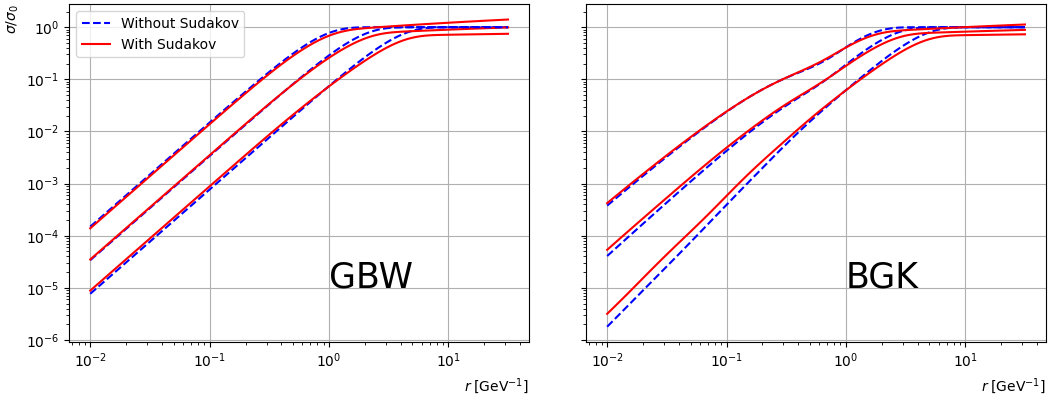
\includegraphics[width=\textwidth]{./dipole.png}
		\caption{%$\sigma_{\mathrm{dipole}}/\sigma_0$ at $Q^2=100\;\mathrm{GeV^2}$,\\ $x=10^{-2},\;10^{-4},\; 10^{-6}$.% (from bottom to top).
		}
		\label{fig:dipole}
	\end{subfigure}
	\begin{subfigure}{0.49\textwidth}
		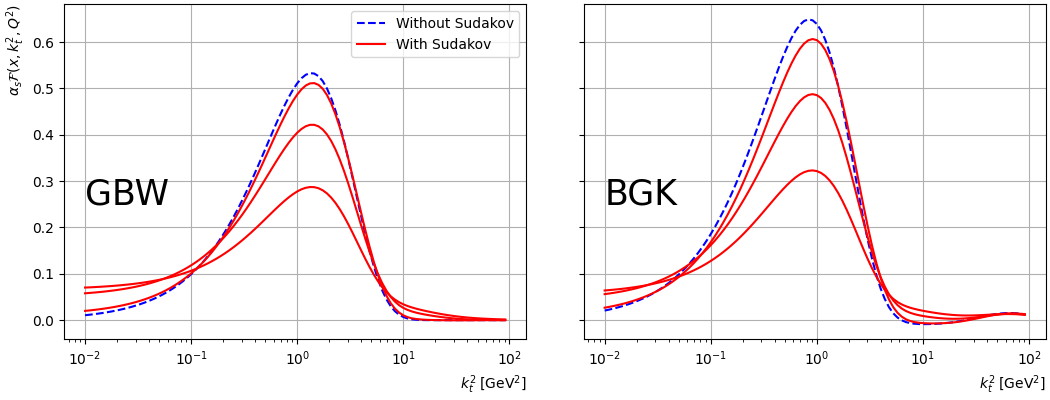
\includegraphics[width=\textwidth]{./gluon.png}
		\caption{%$\alpha_s\mathcal{F}(x,k_t^2,Q^2)$ at $x=10^{-4}$,\\$Q^2=5, \;50 ,\; 500\; \mathrm{GeV^2}$.% (from top to bottom). }%Notice the broadening effect of the Sudakov factor, particularly towards the small value of $k_t^2$.
		}
		\label{fig:gluon}
	\end{subfigure}
	\caption{Left: $\sigma_{\mathrm{dipole}}/\sigma_0$ at $Q^2=100\;\mathrm{GeV^2}$, $x=10^{-2},\;10^{-4},\; 10^{-6}$ (from bottom to top). Right: $\alpha_s\mathcal{F}(x,k_t^2,Q^2)$ at $x=10^{-4}$, $Q^2=5, \;50 ,\; 500\; \mathrm{GeV^2}$ (from top to bottom).
	}
\end{figure*}
\begin{figure*}[t]
	\centering
	\begin{subfigure}{0.49\textwidth}
		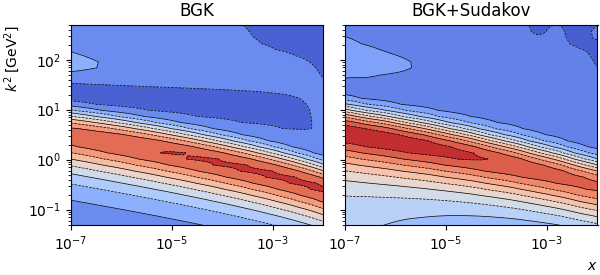
\includegraphics[width=\textwidth]{./BGK-hardscale-175.png}
		%\subcaption{BGK, $Q^2=175\;\mathrm{GeV^2}$}
	\end{subfigure}
	\begin{subfigure}{0.49\textwidth}
		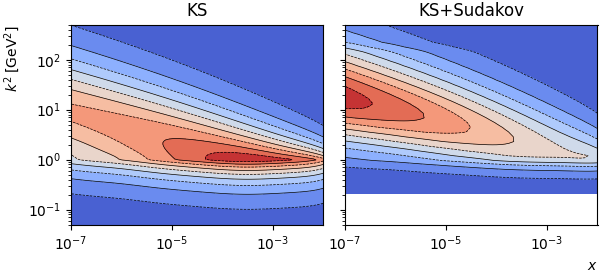
\includegraphics[width=\textwidth]{./KS-hardscale-180.png}
		%\subcaption{KS, $Q^2=180\;\mathrm{GeV^2}$}
	\end{subfigure}
	\caption{Comparisons of hard-scale-independent and hard-scale-dependent gluon densities. }
	\label{fig:3d}
	%\end{figure*}
%\begin{figure*}[t]
%\begin{subfigure}{0.8\textwidth}
%\centering
%   \includegraphics[width=\textwidth]{./critical.png}
%  \caption{Saturation scale $Q_s^2(x)$. The line was plotted for $Q^2=100\;\mathrm{ GeV^2}$.}
% \label{fig:critical}
%    \end{subfigure}
\end{figure*}
\begin{figure*}[t]
	\centering
	\begin{subfigure}{0.49\textwidth}
		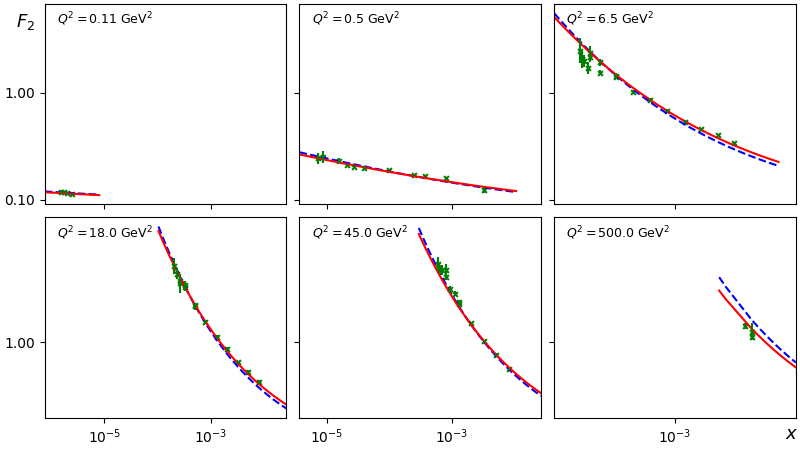
\includegraphics[width=\textwidth]{./F2-data-GBW-lim1.png}
	\end{subfigure}
	\begin{subfigure}{0.49\textwidth}
		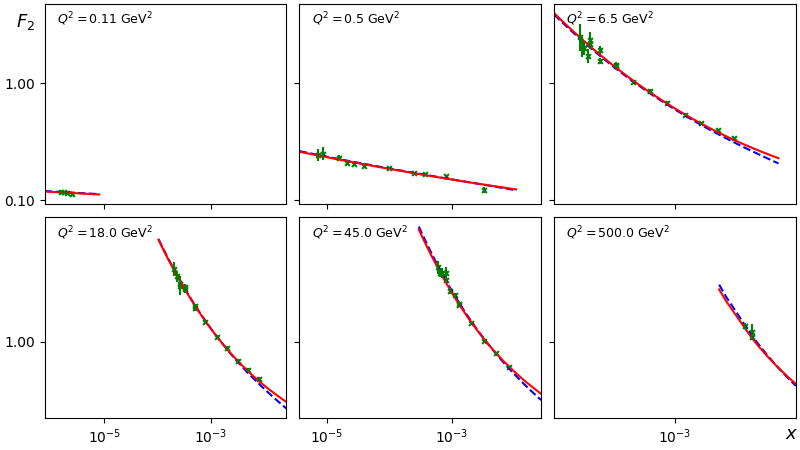
\includegraphics[width=\textwidth]{./F2-data-BGK-lim1.png}
	\end{subfigure}
	\begin{subfigure}{0.45\textwidth}
		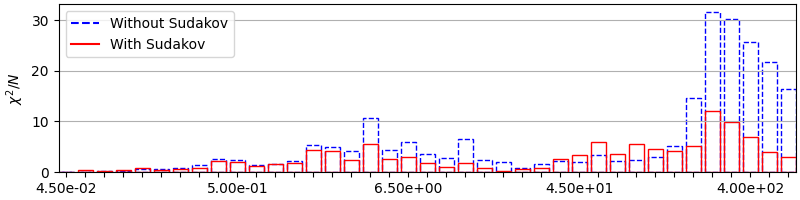
\includegraphics[width=\textwidth]{./F2-data-GBWhist.png}
		\subcaption{GBW}
	\end{subfigure}
	\begin{subfigure}{0.45\textwidth}
		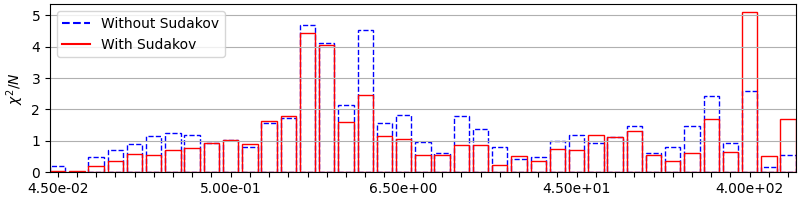
\includegraphics[width=\textwidth]{./F2-data-BGKhist.png}
		\subcaption{BGK}
	\end{subfigure}
	\caption{Top: Comparison of original (dashed blue) and Sudakov-improved (solid red) with  HEAR data (green error bars) at selected $Q^2=0.11,\;0.5,\;6.5,\;18,\;45,\;500\;\mathrm{GeV^2}$. Bottom: $\chi^2/\text{(no. of data)}$ at each $Q^2$.}
	\label{fig:grid}
\end{figure*}
\begin{table*}[t]
	\centering
	\begin{subtable}{0.65\textwidth}
		\centering
		\vspace{1mm}\resizebox{0.75\textwidth}{!}{
		\begin{tabular}{|c|c|c|c|c|}
		\hline
		  &  $\sigma_0 \;[\mathrm{mb}]$ &  $x_0 (10^{-4})$ &  $\lambda$ &  $\chi^2/\mathrm{dof}$ 
		\\\hline
		$\mathrm{GBW}$ & 19.1 & 2.58 & 0.322 & 4.44 \\ \hline
		$\mathrm{GBW+Sud}$& 18.6 & 3.11 & 0.299 & 2.66 \\ \hline
		\end{tabular} 
		}
		\vspace{1mm}
	\end{subtable}

	\centering
	\begin{subtable}{0.65\textwidth}
		\centering
		\vspace{1mm}
		\resizebox{\textwidth}{!}{
		\begin{tabular}{|c|c|c|c|c|c|c|}
		\hline
		&  $\sigma_0\; [\mathrm{mb}]$ &  $A_{\mathrm{g}}$ &  $\lambda_{\mathrm{g}}$ &  $C$ &  $\mu_{0}^2\;[\mathrm{GeV^2}]$ &  $\chi^2/\mathrm{dof}$ 
		\\\hline
		$\mathrm{BGK}$ & 23.3 & 1.18 & 0.0832 & 0.329 & 1.87 & 1.56 \\ \hline
		$\mathrm{BGK+Sud}$ & 22.2 & 8.67 & -0.500 & 0.670 & 3.83 & 1.21 \\ \hline
		\end{tabular} 
		}
		\vspace{1mm}
	\end{subtable}
	\caption{ The parameters and $\chi^2$ per degrees of freedom of the GBW and BGK models (with and without the Sudakov factor, Eq.~(\ref{eq:sudakov})) for cases with mssless light quarks.}
	\label{table:fitresults}
	\vspace{2mm}
	\centering
	\begin{subtable}{0.33\textwidth}
		\centering 
		\resizebox{\textwidth}{!}{
		\begin{tabular}{|c|c|c|}
		\hline
		$Q_{\mathrm{up}}^2 \;[\mathrm{GeV^2}]$&  GBW & GBW+Sud 
		\\\hline
		5 & 1.55 & 1.55 \\ \hline
		%25 & 1.46  & 1.41 \\ \hline
		50 & 1.97  & 1.83 \\ \hline
		%100 & 2.36  & 2.15 \\ \hline
		650 & 4.44  & 2.66 \\ \hline
		\end{tabular} 
		}
	\end{subtable}
	\hspace{4mm}
	\begin{subtable}[t]{0.33\textwidth}
		\resizebox{\textwidth}{!}{
		\begin{tabular}{|c|c|c|}
		\hline
		$Q_{\mathrm{up}}^2 \;[\mathrm{GeV^2}]$&  BGK & BGK+Sud
		\\\hline
		5 & 1.63  & 1.59 \\ \hline
		%25 & 1.42 & 1.30 \\ \hline
		50 & 1.52  & 1.23 \\ \hline
		%100 & 1.55  & 1.25 \\ \hline
		650 & 1.56  & 1.21 \\ \hline
		\end{tabular}
		}
	\end{subtable}
	\caption{Comparison of the quality of fits with different upper limits $Q^2_{\mathrm{up}}\; \mathrm{[GeV^2]} $ of the hard scale. }
	\label{table:Qup}
\end{table*}
\section{Results}
The parameters in the Sudakov form factor is fixed at $C=(2^{-\gamma_E})^2\approx1.26$ and $\mu_{0S}^2=2\mathrm{GeV^2}$, and hence no new fit parameters are needed.
The parameters of GBW and BGK models $\{\sigma_0, x_0,\lambda\}$ and $\{\sigma_0,A_g,\lambda_g,C,\mu_0\}$ respectively are fitted to the HERA data~\cite{Abt:2017nkc} with $x<10^{-2}$ and $0.045\mathrm{GeV^2}\leq Q^2\leq 650\mathrm{GeV^2}$. % using MINUIT package~\cite{minuit}. 
As it was the case for Ref.~\cite{Golec-Biernat:2017lfv}, the fit qualities are better for the cases with massless light quarks, therefore we only present the results with the massless light quarks. Since for the range of $Q^2$ we are interested,  $c$, $b$ quarks contribute, and thus they are included with mass $m_c=1.3\;\mathrm{GeV}$, and $m_b=4.6\;\mathrm{GeV}$ respectively. The choice of  $\mu_{0S}^2$ is somewhat arbitrary, however, preliminary fits showed, for sufficiently small value of $\mu_{0S}^2$, the contribution of the non-perturbative Sudakov factor can be neglected. %Therefore, while it is interesting to see that non-perturbative Sudakov factor indeed compensates for the effect of $\mu_{0S}^2$, for simplicity, we chose $\mu_{0S}^2=2$.\\
The results of the fits are presented in Tab.~\ref{table:fitresults}. One can see that both the GBW and BGK models have improved considerably. One noticeable change in the parameters is that $\lambda_g$ of BGK model has become negative. As discussed in~\cite{Bartels:2002cj} this implies that the strong rise of the integrated gluon density, $g(x,\mu^2)$, at small $x$  is solely due to DGLAP evolution. While the full result of Tab.~\ref{table:fitresults} is fitted to the data $Q^2<650\mathrm{GeV}^2$,  Tab.~\ref{table:Qup} shows the fit results with several upper limit of $Q^2$, $Q_\mathrm{up}^2$. This clearly shows that the Sudakov-improved models have better tolerance for a wide range of $Q^2$. Particularly the fit quality of the BGK model no longer deteriorates as the range of $Q^2$ increases.
Fig.~\ref{fig:dipole} shows the comparison of the  GBW and BGK models with their Sudakov improved versions. The initial suppression and the logarithmic rise at large-$r$ region is due to the Sudakov factor, while the differences in the small-$r$ region are solely due to the changes in the parameters, thus remain in the small-$Q^2$ limit.
Fig.~\ref{fig:gluon} shows that the incorporation of the Sudakov factor smears out the unintegrated gluon density. Consequently, $\alpha \mathcal{F}(x,_t^2 Q^2) $ no longer vanishes in the limit  $k_t^2\rightarrow 0$, which is directly related to the logarithmic rise of the dipole cross section.  While the shape of the gluon density changes, the peaks are located at the same place for various  $Q^2$, indicating little effect to the saturation scale. %(Fig.~\ref{fig:critical}).
Furthermore, one notices in Fig.~\ref{fig:3d} that the differences in the gluon density of the BGK model with and without the Sudakov factor are qualitatively similar to those of Kutak-Sapeta~(KS) gluon distribution~\cite{vanHameren:2020rqt} with and without the Sudakov effects.
Fig.~\ref{fig:grid} shows comparison of the $ F_2$ structure function computed from the models and the HERA data at selected value of $Q^2$, and the $\chi^2/\text{(no. of data)}$ at each $Q^2$. One can see for the GBW model the main improvement is from the large-$Q^2$ region. As for the BGK model one can see in the moderate-$x$ region ($\sim 10^{-2}$), the curve is slightly lifted and fits better with the data.  
%%%%%%%%%%%%%%%%%%%%%%%%%%%%%%%%%%%%%%
%\begin{table}[H]
%\centering
%    \begin{subtable}[H]{0.45\textwidth}
%        \centering
%        \resizebox{\textwidth}{!}{
%           % \begin{tabular}{|c|c|c|}
\hline
	$\mu_{0\mathrm{S}}^2[\mathrm{GeV^2}]$ & $\mathrm{GBWS_{pert}}$ &  $\mathrm{GBWS_{np}}$\\\hline
 1 & 2.71 & 2.72 \\\hline
 2 & 2.66 & 2.67 \\\hline
 3 & 2.64 & 2.65 \\\hline
 4 & 2.64 & 2.64 \\\hline
 5 & 2.64 & 2.65 \\\hline
 \end{tabular} 

%            \begin{tabular}{|c|c|c|}
%\hline%
%\footnotesize	$\mu_{0S}^2[\mathrm{GeV^2}]$ & \footnotesize $\mathrm{GBW+Sud_{pert}}$ & \footnotesize $\mathrm{GBW+Sud_{pert+np}}$\\\hline
% 1 & 2.71 & 2.72 \\\hline
% 2 & 2.66 & 2.67 \\\hline
% 3 & 2.64 & 2.65 \\\hline
% 4 & 2.64 & 2.64 \\\hline
% 5 & 2.64 & 2.65 \\\hline
% \end{tabular} 
%        }
%        \hspace{3mm}
%    \end{subtable}
%    \begin{subtable}[H]{0.45\textwidth}
%        \resizebox{\textwidth}{!}{
%            %\begin{tabular}{|c|c|c|}
\hline
	$\mu_{0\mathrm{S}}^2[\mathrm{GeV^2}]$ & $\mathrm{BGKS_{pert}}$ &  $ \mathrm{BGKS_{np}}$\\\hline
 1 & 1.18 & 1.17 \\\hline
 2 & 1.21 & 1.17 \\\hline
 3 & 1.25 & 1.21 \\\hline
 4 & 1.29 & 1.21 \\\hline
 5 & 1.32 & 1.22 \\\hline
 \end{tabular} 

%\begin{tabular}{|c|c|c|}
%\hline
%\footnotesize	$\mu_{0S}^2[\mathrm{GeV^2}]$ & \footnotesize$\mathrm{BGK+Sud_{pert}}$ & \footnotesize $ \mathrm{BGK+Sud_{pert+np}}$\\\hline
% 1 & 1.18 & 1.17 \\\hline
% 2 & 1.21 & 1.17 \\\hline
% 3 & 1.25 & 1.21 \\\hline
% 4 & 1.29 & 1.21 \\\hline
% 5 & 1.32 & 1.22 \\\hline
% \end{tabular} 
%        }
%    \end{subtable}
%    \caption{$\chi^2/\mathrm{dof}$ of fits with and without the non-perturbative Sudakov factor, with 5 values of $\mu_{0S}^2$ for the Sudakov factor. It is clear that when $\mu_{0S}^2$ is set small, the effect of non-perturbative Sudakov factor is negligible. It is interesting to see that, for the BGK model, inclusion of the non-perturbative factor indeed weakens the dependence on the choice of $\mu_{0S}$.}
%	    \label{table:Snp}
%	    \vspace{3mm}
%\end{table}
 %%%%%%%%%%%%%%%%%%%%%%%%%%%%%%%%%%%%%%%%%%%%%%%%%%%%5   
%
 %%%%%%%%%%%%%%%%%%%%%%%%%%%%%%%%%%%%%%%%%%%%%%%%%%%%

\section{Conclusion}
We have incorporated the Sudakov form factor into the GBW and BGK saturation models. The results of fitting to the HERA data shows considerable improvements for both the models. The Sudakov-improved GBW model can describe the higher-$Q^2$ region better, and the BGK model shows better fit with the data in the moderate-$x$ region. More details can be found in the forthcoming publication Ref.~\cite{Goda:2022wsc}.\\
\section*{Acknowledments}
The research was conducted under a collaboration with S. Sapeta and K. Kutak. The project is partially supported by the European Union’s Horizon 2020 research and innovation program under grant agreement No. 824093, and the author is supported by the Polish National Science Centre grant no. 2017/27/B/ST2/02004.
\printbibliography


\end{document}
